\documentclass[10pt,a4paper]{article}

\usepackage[utf8]{inputenc}
\usepackage[T1]{fontenc}
\usepackage[brazilian]{babel}
\usepackage[a4paper,margin=2cm]{geometry}
\usepackage{booktabs}
\usepackage{graphicx}
\usepackage{amsmath}
\usepackage{hyperref}
\usepackage{xcolor}

\title{Alerta antecipado de picos de consumo de um motor por aprendizagem de máquina}
\author{\textit{[Inserir nomes dos autores]}\\
\small [Instituição / disciplina]}
\date{\today}

\begin{document}
\maketitle

\begin{abstract}
% Este trabalho investiga se sinais operacionais de um veículo permitem antecipar picos de consumo do motor. Foram analisados quatro ensaios, com avaliação leave-one-experiment-out e horizonte de cinco segundos. O Gradient Boosting com atributos operacionais obteve PR-AUC média de 0{,}837 (IC 95\% por bootstrap de episódios: 0{,}793--0{,}867) e PR-AUC de 0{,}589 para identificar o início dos picos. Com custo relativo de três para picos não avisados, 82{,}2\% dos episódios foram antecipados, com antecedência mediana de 3{,}25 s e 55{,}97 alarmes falsos por hora. Os resultados indicam capacidade preditiva nos ensaios disponíveis, mas a validação em apenas quatro ensaios e a unidade física não verificada limitam a generalização e a interpretação prática.
    O objetivo deste trabalha é investigar se sinais operacionais coletados a partir do barramento CAN de experimentos dirigindo um ônibus em uma trajetória específica podem antecipar picos no consumo de combustível do motor. Foram analisados quatro ensaios, com avaliação leave-one-experiment-out e horizonte de cinco segundos. O Gradient Boosting com atributos operacionais obteve PR-AUC média de 0{,}837 (IC 95\% por bootstrap de episódios: 0{,}793--0{,}867) e PR-AUC de 0{,}589 para identificar o início dos picos. Os resultados indicam potencial preditivo a partir dos dados dos ensaios, mas existem limitações nos modelos e na disponibilidade de dados para os experimentos.
\end{abstract}

\noindent\textbf{Palavras-chave:} séries temporais; classificação; alerta antecipado; consumo de motor; Gradient Boosting.

\section{Introdução e objetivo}
Picos de consumo podem sinalizar períodos de elevada demanda do motor. Detectá-los com antecedência pode apoiar decisões do condutor ou de um sistema de controle, desde que o aviso chegue a tempo e o custo de alarmes falsos seja aceitável.

Este trabalho investiga a seguinte pergunta: \emph{é possível prever, a partir de sinais operacionais registrados no barramento CAN de um ônibus, que o consumo entrará em pico nos próximos cinco segundos? Qual é o compromisso entre antecipar episódios e gerar alarmes falsos?} O objetivo é comparar modelos de aprendizagem de máquina com referências simples e avaliar seu desempenho em ensaios não vistos no treinamento.


\section{Dados}
\subsection{Origem, cobertura e variáveis}
Neste estudo, utilizamos dados coletados do barramento CAN de um ônibus conduzido por dois condutores, em dias distintos e sob condições semelhantes. Os dados têm taxa de amostragem de uma amostra por segundo. A Tabela~\ref{tab:variaveis} descreve os campos registrados e as unidades indicadas nos metadados; a Tabela~\ref{table_dados} resume a cobertura dos ensaios. Os arquivos foram fornecidos para este projeto e não têm documentação pública identificada \cite{dadosprojeto}.

Os arquivos fornecidos identificam quatro ensaios e dois dias distintos, mas não registram datas de calendário; portanto, não é possível informar o período cronológico exato. A Tabela~\ref{table_dados} contabiliza as amostras originais, antes da remoção de linhas sem atributos ou rótulos válidos para cada experimento.

\begin{table}[ht]
\centering
\scriptsize
\caption{Variáveis registradas, descrição e unidade indicada nos metadados.}\label{tab:variaveis}
\begin{minipage}[t]{0.49\linewidth}\vspace{0pt}\centering
\begin{tabular}{@{}p{0.13\linewidth}p{0.62\linewidth}p{0.13\linewidth}@{}}
\toprule Variável & Descrição & Unidade \\
\midrule
\texttt{Temp} & Tempo / índice temporal da amostra & s \\
\texttt{Velo} & Velocidade do veículo & m/s \\
\texttt{Acc} & Posição do pedal do acelerador & \% \\
\texttt{Brake} & Posição do pedal de freio & \% \\
\texttt{Gear} & Marcha selecionada (categórica) & 1 \\
\texttt{n} & Rotação do motor & 1/s \\
\texttt{Tau} & Torque do motor & N\,m \\
\texttt{Diem} & Taxa de injeção de combustível & m$^3$/s$^\dagger$ \\
\texttt{Taccm} & Taxa de consumo de combustível & m$^3$/s$^\dagger$ \\
\bottomrule
\end{tabular}
\end{minipage}\hfill
\begin{minipage}[t]{0.49\linewidth}\vspace{0pt}\centering
\begin{tabular}{@{}p{0.13\linewidth}p{0.62\linewidth}p{0.13\linewidth}@{}}
\toprule Variável & Descrição & Unidade \\
\midrule
\texttt{TeLam} & Temperatura do líquido de arrefecimento & K \\
\texttt{Teom} & Temperatura do óleo do motor & K \\
\texttt{Team} & Temperatura ambiente & K \\
\texttt{x} & Distância percorrida pelo veículo & m \\
\texttt{zAl} & Altitude indicada pelo GPS & m \\
\texttt{yLa} & Distância vetorial associada à latitude & m \\
\texttt{xLo} & Distância vetorial associada à longitude & m \\
\texttt{mass} & Massa por eixo & kg \\
\bottomrule
\end{tabular}
\end{minipage}
\end{table}
\noindent{\scriptsize $^\dagger$ Unidade declarada nos metadados, mas não validada independentemente; os resultados de consumo são apresentados em unidades originais (u.o.).}

\begin{table}[ht]
\centering
\small
\caption{Cobertura e definição de pico por ensaio. Cada linha representa uma amostra por segundo.}
\label{table_dados}
\begin{tabular}{lrrrrr}
\toprule
Ensaio & Amostras & Duração (h) & Limiar (u.o.) & Episódios & Mediana (s) \\
\midrule
D1T1A & 1.984 & 0{,}551 & 32{,}720 & 53 & 3 \\
D1T1B & 1.776 & 0{,}493 & 33{,}875 & 47 & 2 \\
D1T2  & 3.876 & 1{,}077 & 29{,}000 & 72 & 3 \\
D2T1  & 1.703 & 0{,}473 & 30{,}060 & 63 & 2 \\
\midrule
Total & 9.339 & 2{,}594 & -- & 235 & -- \\
\bottomrule
\end{tabular}
\end{table}
Cada amostra corresponde a um segundo; as contagens da Tabela~\ref{table_dados} referem-se aos registros originais, antes da seleção de linhas válidas para cada modelo.


\subsection{Alvo e análise exploratória}

Em cada ensaio, define-se como pico qualquer segundo em que o consumo excede o percentil 90 daquele próprio ensaio como mostrado na figura \ref{fig_pico} 
Uma sequência de segundos consecutivos acima do limiar forma um episódio. Para classificação, o alvo vale um quando ocorre ao menos um segundo de pico 
nos cinco segundos seguintes ($t_{+1}$ a $t_{+5}$); o instante atual não integra o horizonte. A prevalência desse alvo variou de 14{,}9\% a 19{,}6\% entre ensaios.

\begin{figure}[ht]
\centering
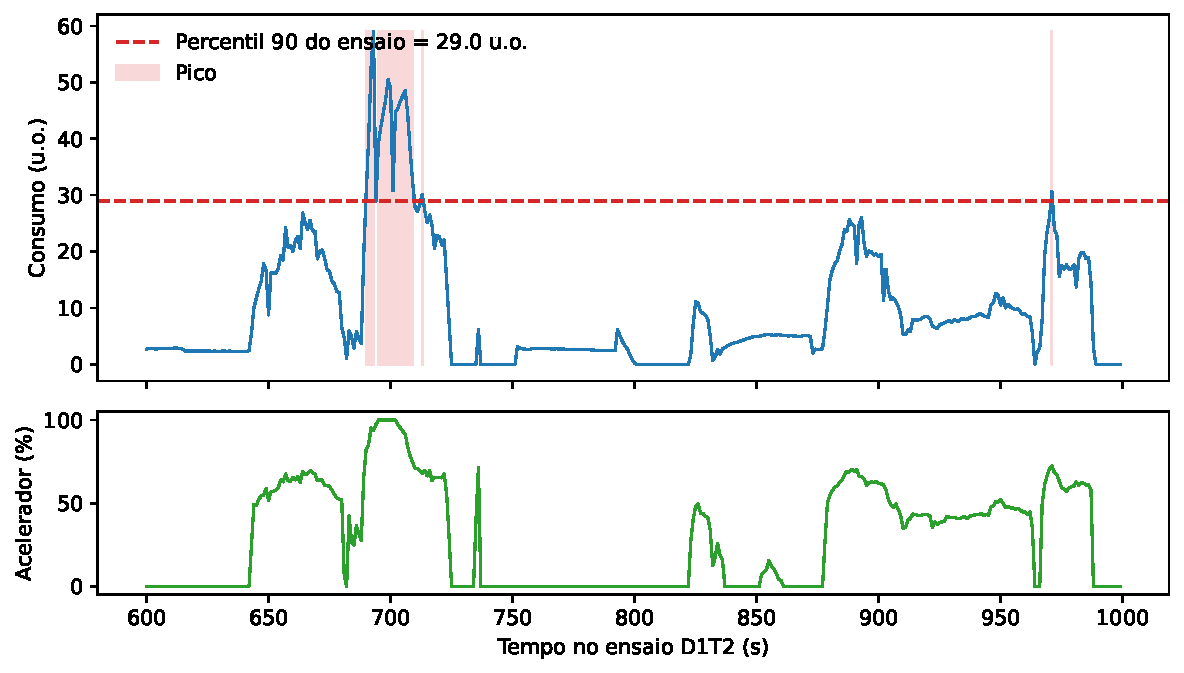
\includegraphics[width=0.86\linewidth]{figures/fig_pico.pdf}
\caption{Exemplo de episódio de pico no ensaio D1T2. O limiar é o percentil 90 do consumo desse ensaio; o painel inferior mostra o acelerador no mesmo intervalo.}
\label{fig_pico}
\end{figure}

O limiar correspondente ao percentil 90 variou de 29{,}00 a 33{,}88 unidades originais; foram observados de 47 a 72 episódios por ensaio, com duração mediana de 2 a 3 segundos. A análise exploratória também mostra aumento de acelerador, torque, rotação e velocidade à medida que se aproxima o início dos episódios. Essa associação é descritiva e não estabelece causalidade.


% \paragraph{Limitação de unidade e tratamentos.} Embora o cabeçalho da coluna indique m$^3$/s, a escala observada não é compatível com a variável de injeção disponível, e a unidade não foi validada. Por isso, os valores são reportados em unidades originais (u.o.); MAE e RMSE dependem dessa escala. \textbf{[Completar: origem e tratamento de valores ausentes, sincronização, filtragem e eventuais exclusões de linhas.]}

\section{Metodologia}
\subsection{Preparação, modelos e avaliação}

Em uma etapa exploratória complementar, foram gerados 13 grupos adimensionais de Buckingham a partir de 17 variáveis e uma matriz dimensional de posto 4 (17 menos 4 = 13). Contudo, esses 13 grupos não são entradas dos classificadores avaliados neste artigo: o notebook de alerta usa atributos operacionais construídos diretamente a partir dos sinais medidos. A comparação específica com temperatura do óleo inclui essa temperatura e o grupo derivado $\pi_7$ (óleo dividido pela temperatura do líquido de arrefecimento).

A temperatura do óleo está disponível em três dos quatro ensaios (D1T1A, D1T1B e D1T2) e ausente em D2T1. Por isso, os experimentos principais a desconsideram, e a análise de ganho com óleo é feita separadamente nos três ensaios com medição, mantendo $\pi_7$ junto com a temperatura.

As séries foram ordenadas por amostra dentro de cada ensaio. Atributos derivados incluem diferenças em 1 e 3 s, médias móveis de 5 s e janelas dos últimos 10 s; os alvos futuros foram construídos sem atravessar os limites dos ensaios. Para cada tarefa, foram removidas linhas sem os atributos ou rótulos requeridos, sem imputação. O alerta principal usa atributos operacionais e não inclui consumo atual ou passado como preditor. Foram comparados regressão logística padronizada (até 3.000 iterações), HGB e uma CNN 1D com janelas de 10 s, além de persistência e uma regra Apriori como referências. O HGB usa profundidade máxima 4, taxa de aprendizado 0{,}05 e 200 iterações \cite{friedman2001}; a CNN tem duas convoluções de 16 filtros, normalização por canal usando apenas o treino, Adam, taxa 0{,}002, lotes de 256, peso de decaimento $10^{-4}$, 30 épocas fixas e média de três sementes. Não foi feito ajuste extensivo de hiperparâmetros. Para regressão em $t+5$, comparam-se persistência, HGB com perda absoluta (profundidade 4, taxa 0{,}05, 300 iterações) sobre a variação do consumo, modelos por regime (K-Means com seis clusters, escalonados no treino, e fallback global abaixo de 200 observações) e uma combinação híbrida que recorre à persistência quando o valor atual supera o limiar calculado apenas no treino. Os intervalos de regressão usam quantis 0{,}1/0{,}5/0{,}9 e ajuste conformal com previsões internas.

A avaliação principal deixa um ensaio inteiro de fora por vez (leave-one-experiment-out, quatro folds). Calibração isotônica e seleção do limiar usam somente previsões internas fora da amostra nos ensaios de treino. O limiar é escolhido numa grade de 45 valores entre 0{,}02 e 0{,}90 para minimizar $C_{FA}$ por amostra de decisão com falso alerta mais $C_{MISS}$ por amostra positiva sem alerta; essa contagem usa o rótulo de ocorrência nos cinco segundos futuros, não a duração física exata do episódio. O caso principal usa $C_{FA}=1$ e $C_{MISS}=3$, com sensibilidades em 1 e 10. Uma validação secundária usa cinco blocos temporais e purga de 10 s ao redor de cada bloco de teste.

As métricas de classificação incluem PR-AUC (área sob a curva precisão--revocação), PR-AUC nas linhas fora de pico, precisão, recall, episódios antecipados, antecedência mediana e alarmes falsos por hora. Para regressão reporta-se MAE geral e nos segundos que serão pico. Intervalos de confiança de 95\% e diferenças pareadas são estimados por bootstrap de blocos/episódios (400 reamostragens, semente 42); esses intervalos não quantificam plenamente a variação entre ensaios. A robustez é examinada para percentis 85/90/95 e horizontes de 3/5/10 s. A implementação usa Python, scikit-learn e PyTorch; entre outras dependências, pandas, NumPy e mlxtend.

\subsection{Ferramentas}
Os experimentos foram executados em notebook Jupyter com Python 3.14.2, scikit-learn 1.9.1 e PyTorch 2.14.1. A PR-AUC foi adotada por ser informativa em classificação com classes desbalanceadas; a calibração isotônica converte as pontuações em probabilidades para selecionar o limiar operacional \cite{davis2006,niculescu2005}.

\section{Resultados e discussão}
\subsection{Desempenho de classificação}
\begin{table}[ht]
\centering
\small
\caption{Desempenho médio nos quatro ensaios deixados de fora, conforme resultados registrados no notebook.}
\begin{tabular}{lcc}
\toprule
Abordagem & PR-AUC & PR-AUC no início \\
\midrule
Persistência & 0{,}550 & 0{,}091 \\
Regra Apriori & 0{,}303 & 0{,}156 \\
Regressão logística (janela) & 0{,}837 & 0{,}563 \\
HGB (janela) & 0{,}828 & 0{,}550 \\
HGB (atributos operacionais) & 0{,}837 & 0{,}589 \\
CNN 1D (janela) & 0{,}830 & 0{,}528 \\
\bottomrule
\end{tabular}
\end{table}

\begin{table}[ht]
\centering
\small
\caption{Compromisso operacional do alerta no teste por ensaio. A antecedência é calculada apenas nos episódios isolados.}
\label{tab:alerta}
\begin{tabular}{lrrrr}
\toprule
Alerta & Precisão & Recall & Falsos/h & Antecipados; mediana (s) \\
\midrule
Persistência & 0{,}887 & 0{,}526 & 17{,}10 & 0\%; -- \\
Regra Apriori & 0{,}688 & 0{,}250 & 38{,}32 & 63{,}1\%; 2{,}63 \\
HGB, $C_{MISS}=1$ & 0{,}778 & 0{,}683 & 39{,}70 & 68{,}3\%; 2{,}75 \\
HGB, $C_{MISS}=3$ & 0{,}663 & 0{,}822 & 55{,}97 & 92{,}0\%; 3{,}25 \\
HGB, $C_{MISS}=10$ & 0{,}489 & 0{,}927 & 107{,}08 & 100\%; 4{,}75 \\
\bottomrule
\end{tabular}
\end{table}

Na regressão, os seis modelos por regime K-Means tiveram MAE geral de 5{,}285 u.o., contra 5{,}064 do HGB global e 5{,}435 da persistência, portanto não trouxeram ganho sobre o modelo global. Separadamente, na análise descritiva com oito regimes ajustados sobre o conjunto completo, os dois regimes de maior risco apresentaram prevalências de 0{,}57 e 0{,}37, ante 0{,}17 no conjunto; ao menos um deles ocorreu nos cinco segundos anteriores a 54\% dos 85 inícios isolados. Regra Apriori ou regime de risco identificou 82\% desses inícios. Essa análise é exploratória, não uma validação preditiva, e não demonstra causalidade.

Também foi avaliado o ganho de informação da temperatura do óleo, comparando as mesmas linhas e folds nos três ensaios que a medem. A inclusão da temperatura e de $\pi_7$ não melhorou as métricas médias: PR-AUC no início passou de 0{,}528 para 0{,}506, e a diferença pareada foi $-0{,}020$ (IC 95\%: $-0{,}046$ a $0{,}002$). Como o intervalo inclui zero e há apenas três folds, não se conclui que a variável seja inútil; neste conjunto, não há evidência clara de ganho.

HGB com atributos operacionais apresentou a maior PR-AUC no início do pico (0{,}589; IC 95\%: 0{,}532--0{,}656), embora sua PR-AUC global tenha empatado, após arredondamento, com a regressão logística. A CNN não superou o HGB operacional: a diferença pareada de PR-AUC no início foi $-0{,}057$ (IC 95\%: $-0{,}097$ a $-0{,}023$). Isso sugere que, neste conjunto pequeno, os atributos operacionais explícitos são competitivos com entradas temporais mais complexas.

\subsection{Operação do alerta e regressão}
A Tabela~\ref{tab:alerta} evidencia o compromisso operacional: penalizar mais os picos não avisados aumenta recall e antecedência, ao custo de menor precisão e mais alarmes falsos. A persistência é precisa, mas só alerta após o início; a regra Apriori tem recall baixo. Os custos são hipotéticos e o limiar deve ser definido para a aplicação real.

Na regressão, o HGB global reduziu o MAE geral de 5{,}435 (persistência) para 5{,}064 u.o., mas aumentou o MAE nos segundos que seriam pico de 11{,}843 para 14{,}177 u.o. A variante híbrida reduziu esse erro em picos para 12{,}391 u.o., ainda acima da persistência. O intervalo conformalizado, nominalmente de 80\%, cobriu 80{,}6\% dos casos gerais, mas apenas 53{,}9\% dos segundos de pico (largura média 16{,}46 u.o.); o intervalo quantílico sem conformalização cobriu 72{,}8\% e 51{,}9\%, respectivamente. A conformalização ajusta os limites quantílicos com erros obtidos por validação interna \cite{romano2019}. A unidade não validada impede interpretar esses erros em escala física.

\subsection{Robustez e limitações da evidência}
Na grade de percentis e horizontes, a PR-AUC do modelo variou de 0{,}659 a 0{,}889 e permaneceu acima da persistência (0{,}381 a 0{,}654). O melhor resultado ocorreu com percentil 85 e horizonte de 3 s; o menor, com percentil 95 e horizonte de 10 s, mostrando que a definição mais rara e o horizonte maior tornam a tarefa mais difícil. A validação em blocos temporais obteve PR-AUC média 0{,}836, próxima à validação por ensaio; ela é menos exigente, pois compartilha o contexto de condução entre treino e teste. A comparação pareada da temperatura do óleo está descrita acima.

Os sinais de acelerador e torque tiveram maior importância por permutação (queda média de PR-AUC de 0{,}480 e 0{,}185 ao embaralhar cada grupo), coerente com a elevação de acelerador, torque, rotação e velocidade observada antes dos picos. Regras e regimes também capturam parte dos episódios. Essas análises descrevem associações, não causas. As limitações centrais são quatro ensaios de um único ônibus, dois condutores, uma trajetória e apenas uma taxa de amostragem (1 Hz); os intervalos por bootstrap de episódios não representam a variação entre veículos, trajetórias ou ensaios. A unidade do consumo permanece não validada e os falsos alarmes podem ser excessivos para uso operacional.

\section{Conclusão}
Nos quatro ensaios, HGB com atributos operacionais foi a abordagem mais adequada para identificar inícios; a CNN não demonstrou ganho. O alerta antecipa episódios, mas gera falsos alarmes, e a regressão continua menos precisa que a persistência dentro dos picos. O objetivo foi alcançado como prova de conceito. O desenvolvimento exigiu conhecimentos de atributos de séries temporais, análise dimensional, calibração e validação sem vazamento. A base pequena, a unidade não verificada, a taxa única de 1 Hz e os custos hipotéticos impedem concluir que a solução esteja pronta para uso. Próximos passos são coletar mais dados em múltiplas trajetórias e taxas de amostragem, validar sensores e custos, e testar a generalização para veículos diferentes e trajetórias não vistas. Até essa validação externa, não se recomenda controle automático.

% As referências não entram no limite de quatro páginas.
\begin{thebibliography}{9}
\bibitem{friedman2001} J. H. Friedman, ``Greedy function approximation: A gradient boosting machine,'' \textit{The Annals of Statistics}, vol. 29, no. 5, pp. 1189--1232, 2001. doi: 10.1214/aos/1013203451.
\bibitem{davis2006} J. Davis and M. Goadrich, ``The relationship between Precision-Recall and ROC curves,'' in \textit{Proceedings of the 23rd International Conference on Machine Learning}, pp. 233--240, 2006. doi: 10.1145/1143844.1143874.
\bibitem{niculescu2005} A. Niculescu-Mizil and R. Caruana, ``Predicting good probabilities with supervised learning,'' in \textit{Proceedings of the 22nd International Conference on Machine Learning}, pp. 625--632, 2005. doi: 10.1145/1102351.1102430.
\bibitem{romano2019} Y. Romano, E. Patterson, and E. Candes, ``Conformalized quantile regression,'' in \textit{Advances in Neural Information Processing Systems}, vol. 32, 2019.
\bibitem{dadosprojeto} Grupo do projeto, ``Medições do barramento CAN de um ônibus em quatro ensaios,'' arquivos \texttt{Dados/Data\_set.CSV} e \texttt{Dados/Data\_set\_param.CSV}, dados não publicados, fornecidos para este estudo.
\end{thebibliography}

\end{document}
